\chapter{Near--Real--Time Data Displays and CLEO Utilities}\label{chap:datadisplay}
 
%++++++++++++++++++++++++++++++++++++++++++++++++++++++++++++++++++++++++++++
\section{The Astrid Data Display Tab}
 
The Data Display Tab provides a real time display of your \gls{GBT} data
so that you can check that you are getting valid data.  The Data
Display is actually running an application called
\glsreset{GFM}\gls{GFM}.  This application provides sub-scan-based
display and analysis of \gls{GBT} data, either in real-time as the data is
being collected, or in an offline mode where it can be used to simply
step through the sub-scans from an observation.  Users are encouraged
to run \gls{GFM} offline for reanalyzing data during observations.  A
separate \gls{GFM} application can be launched from the Linux prompt via the
{\tt gfm} command or \gls{Astrid} could be switched to offline-mode.

\subsection{Working Online}

If you are using either of \gls{Astrid}'s \dq{online} modes (see \S~\ref{sec:astridmode})
and have selected the \dq{DataDisplay} tab, then the data display will update as new data
are obtained. Continuum and Spectral Line data are only updated when these displays are
being viewed. Pointing and Focus data are always automatically updated whether or not
their displays are being shown or not.  Due to this feature, clicking on previous
observations while Pointing and Focus scans are in progress can confuse \gls{GFM} and
should be avoided.  The list of scans will always automatically update.

\subsection{Working Offline}\label{sec:workingOffline}

You can look at data that have already been taken with the \gls{GBT} by running \gls{Astrid} in
its \dq{offline} mode. To view data in this mode you need to follow these steps:

\begin{enumerate}[label=\bfseries{Step \arabic*.},leftmargin=*,itemsep=0pt]
\item Change the \gls{Astrid}\ mode to \dq{offline} (see \S~\ref{sec:astridmode}).
\item Select {\btt File}$\rightarrow${\btt Open} from the drop-down menu in the Data Display Tab.
\item Select a project ID from the list of project directories in {\tt /home/gbtdata/}.
\item Double-click {\tt ScanLog.fits} to access the data.
\item It may take several seconds to a few minutes to access all of your scans depending
on the amount of data to load.  The process is complete when you see a list of scans displayed
sequentially on the left hand side of the \gls{GFM} display.
\item Click on a scan in the scan list window to process it.
\end{enumerate}

\subsection{Pointing and Focus Data Display}\label{sec:pointandfocus}
%
%

Pointing scans (from Peak, AutoPeak and AutoPeakFocus -- see below) will appear under
the Pointing Tab.  If working \dq{Online}, the data display will automatically process
the pointing scans. {\bf Note that clicking on previous scans while Pointing and Focus
scans are in progress may interfere with automatic processing.} It will calibrate the
data, remove a \gls{baseline} and fit a Gaussian to the data.  After the two azimuth
scans it will then automatically update the \gls{GBT} \gls{MC} system with the new azimuth
pointing offset values that it determined. It will then automatically update the
elevation pointing offset after the two elevation scans, unless certain criteria are
not met (see \S~\ref{sec:fittingacceptance}). A sample of the Data Display Application
after a pointing is shown in Figure~\ref{fig:astridpointing}.

\begin{figure}[!h]
\begin{center}
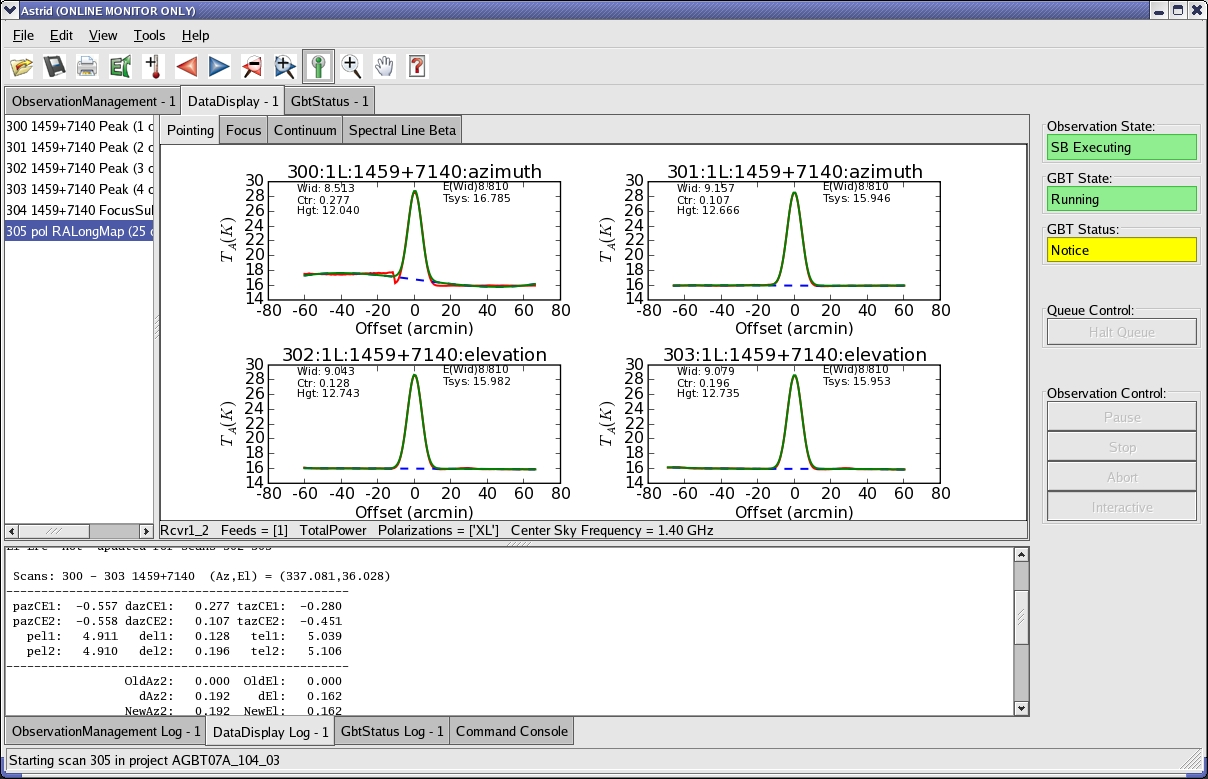
\includegraphics[width=0.6\linewidth]{AstridDataDisplayTabPointing.jpg}
\caption[The Pointing subtab of the Astrid Data Display]
{The Pointing subtab of the \gls{Astrid} Data Display. 
\label{fig:astridpointing} }
\end{center}
\end{figure}

The focus scan data will appear under the Focus Tab; see Figure~\ref{fig:astridfocus}.
Again, if \dq{Online} the data will be processed automatically. They will be calibrated,
have a \gls{baseline} removed and a Gaussian will be fit to the data.  The focus offset
will automatically be sent to the \gls{MC} system.

\begin{figure}[!h]
\begin{center}
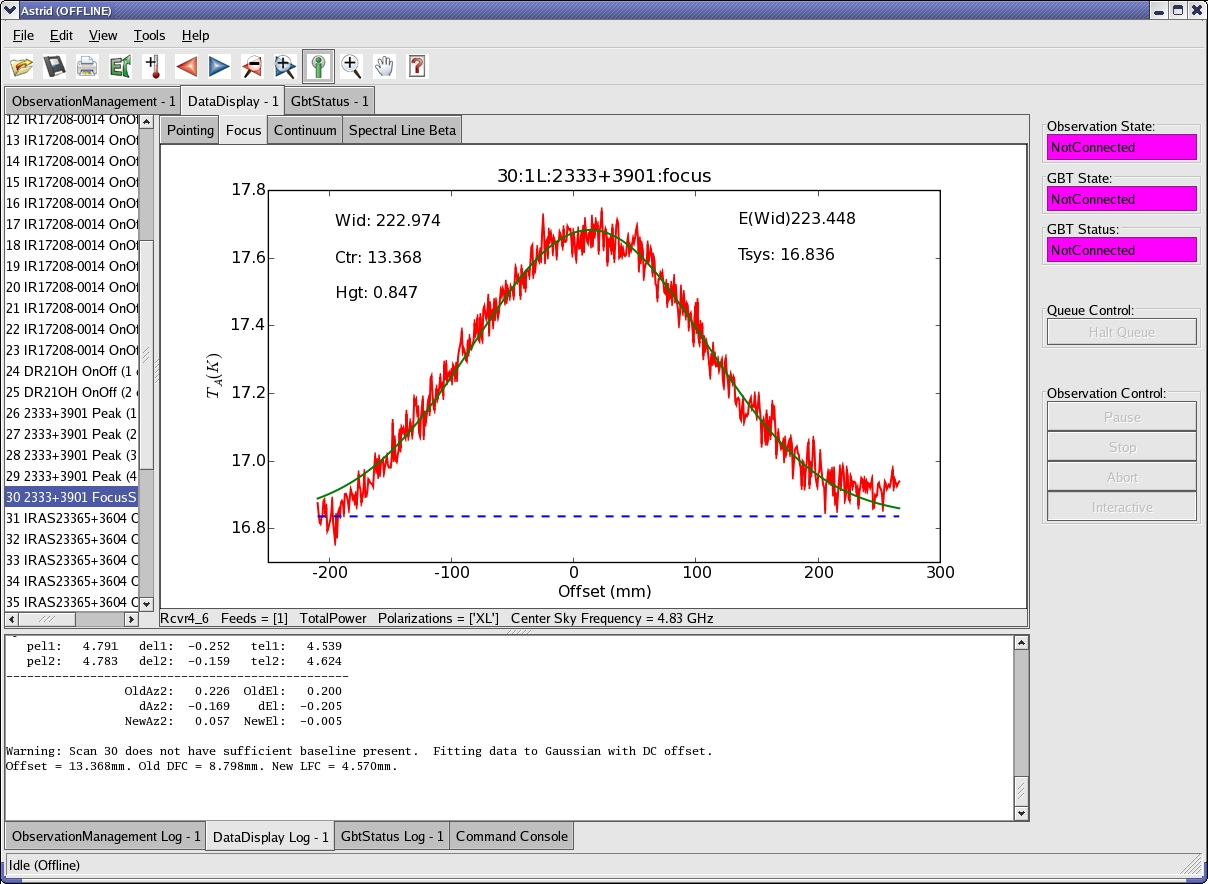
\includegraphics[width=0.6\linewidth]{AstridDataDisplayTabFocus.jpg}
\caption[The Focus subtab of the Astrid Data Display]
{The Focus subtab of the \gls{Astrid} Data Display. 
\label{fig:astridfocus} }
\end{center}
\end{figure}

\noindent The details of pointing and focus observations are described in \S~\ref{sec:utilityscans}.

\newpage

\subsubsection{Fitting Acceptance Options}\label{sec:fittingacceptance}

\gls{GFM} has several levels of determining whether or not the pointing and focus
solutions will be updated in the \gls{MC} system. The expected \gls{FWHM} of the Gaussian
fitted to the observed pointing data as the \gls{GBT} slews across the source should be 
$\sim 748/\nu_{\rm GHz}$\,arc--seconds where $\nu_{\rm GHz}$ is the observing frequency in
GHz.

For a focus scan the resulting data should approximate a Gaussian with a \gls{FWHM} of
$1080\ \nu_{\rm GHz}$, in mm. The default behavior is to asssume that a pointing fit is
bad if the \gls{FWHM} differ from the expected value by more than $30\%$ or if the pointing
correction is more than twice the \gls{FWHM} in magnitude.  The default for a bad focus
scan is if the \gls{FWHM} is more than $30\%$ from the expected value. Users may change
fitting acceptance criteria by: 

\begin{enumerate}[label=\bfseries{Step \arabic*.},leftmargin=*,itemsep=0pt]
\item Select the Pointing or Focus Subtab in the Data Display.
\item Select {\btt Tools}$\rightarrow${\btt Options...} from the drop--down menu.
\item Select the new mode in the \dq{Fitting Acceptance Criteria} tab of the pop--up window.
\item[{\bf NOTE:}] Options must be set independently for both Pointing and Focus
{\bf before} each type of observation in order to take effect.
\end{enumerate}

\noindent \gls{GFM} recognizes the fitting acceptance criteria shown in
Figure~\ref{fig:acceptance} only when \gls{Astrid} is in one of its online modes.
The default setting is to \dq{Automatically accept good fits, automatically reject
bad fits}.  Users may also choose to never apply corrections or interactively accept
bad and/or good fits.  There is also an option to \dq{Accept all automatically} which
can be very dangerous and should only be used by experts.

\vspace{2.5mm}

\noindent\begin{minipage}[t]{0.485\linewidth}
\setlength{\abovecaptionskip}{0pt}\setlength{\belowcaptionskip}{0pt}
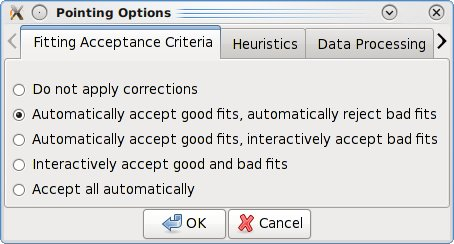
\includegraphics[width=\linewidth]{fittingacceptance.jpg}
\captionof{figure}[Pointing and Focus acceptance pop-up]
{The pop--up menu to change the pointing and focus fitting acceptance criteria. 
\label{fig:acceptance} }
\end{minipage}
\hfill
\begin{minipage}[t]{0.485\linewidth}
\setlength{\abovecaptionskip}{0pt}\setlength{\belowcaptionskip}{0pt}
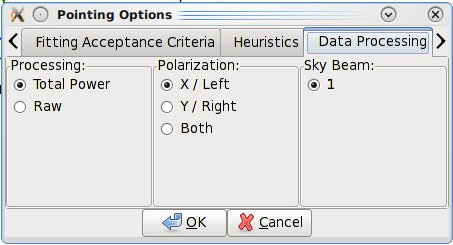
\includegraphics[width=\linewidth]{dataProcessing.jpeg}
\captionof{figure}[Pointing and Focus change fitting pop-up]
{The pop--up menu to change the polarization and calibration used in pointing and
focus fitting. \label{fig:processing} }
\end{minipage}


\subsubsection{Data Processing Options}\label{sec:gfmdataprocessing}

The user may change the data processing strategy, beams, and/or polarizations used 
by \gls{GFM} in reducing pointing or focus scans.  This is not needed typically since the
software picks the proper default settings under normal conditions.  However, for
example, if the X polarization channel is faulty for some reason, one can use the Y
channel instead. This can be done by:

\begin{enumerate}[label=\bfseries{Step \arabic*.},leftmargin=*,%labelindent=\parindent
itemsep=0pt]
\item Select the Pointing or Focus Subtab in the Data Display.
\item Select {\btt Tools}$\rightarrow${\btt Options...} from the drop--down menu.
\item Make new data processing selections in the Data Processing Tab of the pop--up
window (see Figure~\ref{fig:processing}).
\item[{\bf NOTE:}] Options must be set independently for both Pointing and Focus
{\bf before} each type of observation in order to take effect.
\end{enumerate}

\newpage

\subsubsection{Heuristics Options}\label{sec:heuristics}

Heuristics is a generic term used at the \gls{GBT} to quantify the \dq{goodness of fit} of
the pointing and focus data reduction solutions. Based on the known properties of the
\gls{GBT} , parts of the solution, such as the \gls{beamwidth} in pointing data, should
have certain values within measurement errors.  The Heuristics define how large these
errors can be. The user may change the Heuristics by: 

\begin{enumerate}[label=\bfseries{Step \arabic*.},leftmargin=*,
itemsep=0pt]
\item Select the Pointing or Focus Subtab in the Data Display.
\item Select {\btt Tools}$\rightarrow${\btt Options...} from the drop--down menu.
\item Select the new mode in the Heuristics tab of the pop--up window
(see Figure~\ref{fig:heuristic}).
\item[{\bf NOTE:}] Options must be set independently for both Pointing and Focus
{\bf before} each type of observation in order to take effect.
\end{enumerate}

\gls{GFM} allows the observer to switch between \dq{standard}, \dq{relaxed}, and
\dq{user-defined} heuristics.  The \dq{standard} and \dq{relaxed} heuristic values are
predefined and cannot be changed by the user.  Under normal observing conditions the
observer should expect to use the \dq{standard} values.  Under marginal weather
conditions and/or high frequency observations \dq{relaxed} heuristics may be appropriate.
The \dq{user-defined} heuristic values should only be used by experts.  If you wish to
use \dq{user-defined} heuristics then you should contact your \gls{GBT} support scientist.
The default mode is \dq{standard}.

The \dq{standard} heuristics expect that the fitted Gaussians have a \gls{FWHM}
within $30\%$ of the expected values and that the pointing solution is within
twice the \gls{FWHM} of the nominal location of the source.  For the \dq{relaxed}
heuristics this becomes within $50\%$ of the expected \gls{FWHM} of the Gaussian
fits and three times the \gls{FWHM} for the pointing correction.

\vspace{2.5mm}

\noindent\begin{minipage}[t]{0.45\linewidth}
\setlength{\abovecaptionskip}{0pt}\setlength{\belowcaptionskip}{0pt}
\vspace{0pt}
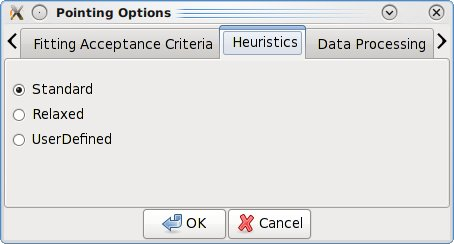
\includegraphics[width=\linewidth]{heuristics.jpg}
\captionof{figure}[Pointing and Focus heuristics pop-up]
{The pop--up menu to change the pointing and focus fitting heuristics.
\label{fig:heuristic} }
\end{minipage}
\hfill
\begin{minipage}[t]{0.45\linewidth}
\setlength{\abovecaptionskip}{0pt}\setlength{\belowcaptionskip}{0pt}
\vspace{0pt}
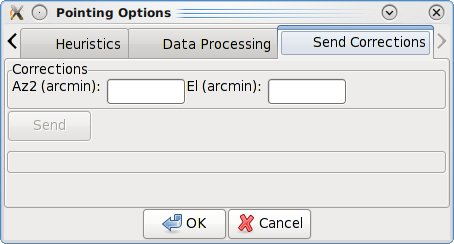
\includegraphics[width=\linewidth]{sendcorrections.jpg}
\captionof{figure}[Send Corrections pop-up]{The pop--up menu to manually send pointing corrections
to the telescope.\label{fig:sendcorrections} }
\end{minipage}

\vspace{-2.5mm}

\subsubsection{Send Corrections}\label{sec:gfmsendcorrections}

For most observations, \gls{GFM} processing produces good fits, and the solutions are
automatically sent to the telescope using the default settings.  However, at high
frequencies (especially \gls{Wband} 68-92 GHz Receiver), fits may fail, and the user may want
to manually send the corrections to the telescope.  The user may tell the operator to
enter a solution, or they can send the corrections themselves using the Send Corrections
tab. Note that corrections show up instantly within the \gls{CLEO} status window
(see \S~\ref{sec:cleo}), but do not take effect until the start of the next scan.
This can be done by:

\begin{enumerate}[label=\bfseries{Step \arabic*.},leftmargin=*,
itemsep=0pt]
\item Select the Pointing or Focus Subtab in the Data Display.
\item Select {\btt Tools}$\rightarrow${\btt Options...} from the drop--down menu.
\item Select the Send Corrections Tab in the pop--up window (if not visible use
arrow button on the right, the Send Corrections tab is farthest to the right)
\item Enter the corrections in the text box, and click \astridbutton{Send} to send the
solutions to the telescope. (see Figure~\ref{fig:sendcorrections}).
\end{enumerate}

\newpage

\subsection{OOF Data Display}\label{sec:oofdatadisplay}

\gls{OOF} is a technique for measuring large-scale errors in the shape of the reflecting
surface by mapping a strong point source both in and out of focus.  The procedure
derives surface corrections which can be sent to the active surface controller to
correct surface errors. The procedure is recommended for high-frequency observing at
frequencies of 30~GHz and higher.

The AutoOOF procedure will obtain three \gls{OTF} maps, each taken at a different focus
position.  Processing will begin automatically upon completion of the third map, the
status of which can be viewed in the progress bar under \dq{AutoOOF Processing Status}
on the right--hand--side of the screen.  Once complete, the result will be displayed
in the \gls{OOF} subtab of the \gls{Astrid} Data Display (see
Figure~\ref{fig:AstridAutoOOF}).

\begin{figure}[!h]
\begin{center}
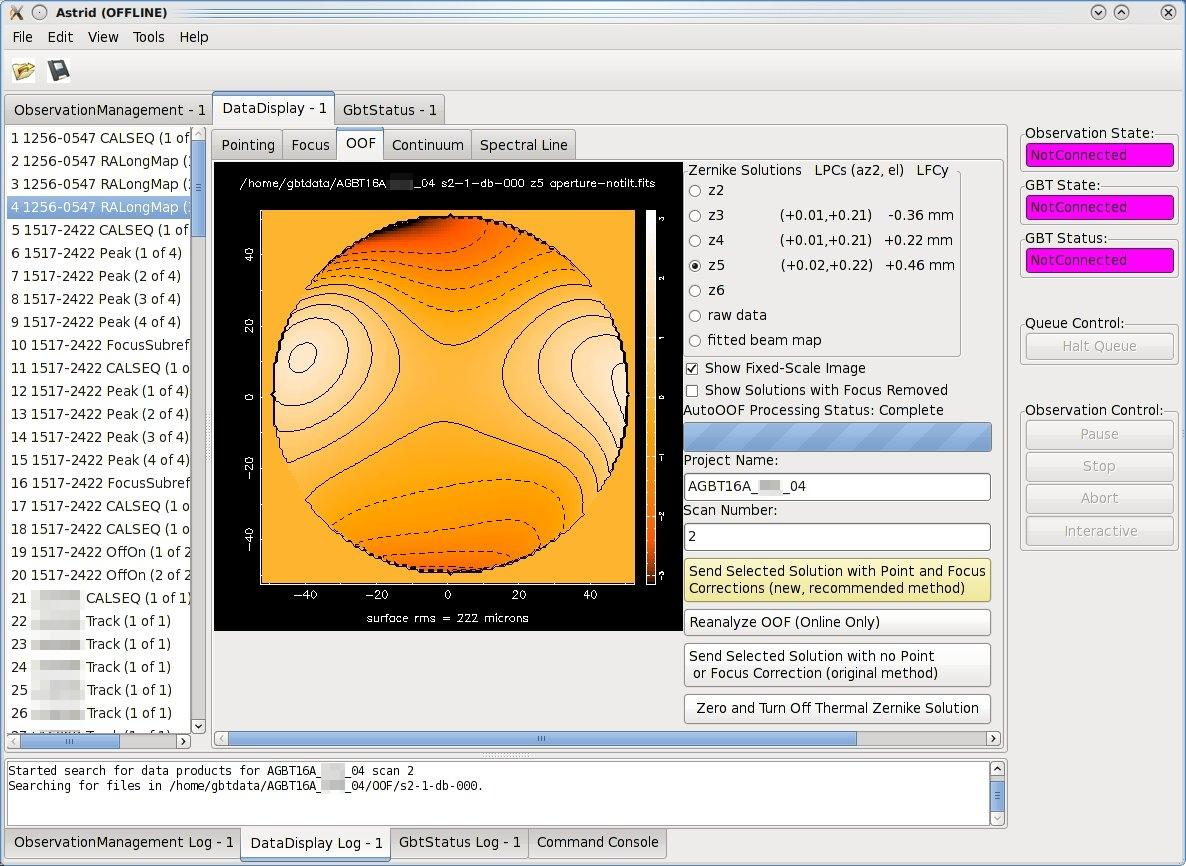
\includegraphics[width=\linewidth]{oof_screen.jpg}
\caption[The OOF subtab of the Astrid Data Display]
{The OOF subtab of the \gls{Astrid} Data Display.\label{fig:AstridAutoOOF} }
\end{center}
\end{figure}

Once processing is complete, the default solution displayed in \gls{Astrid} is the
fifth-order Zernike fit (z5).  The most aggressive fit is z6, while z3 is less
aggressive.  Solutions may be selected and viewed via the radio buttons in the
upper--right section of the screen.  Derived Local Pointing Corrections (LPCs) in
arcminutes, and Local Focus Corrections (LFCy) in millimeters are displayed to the right
of each radio button.  Raw AutoOOF data at each focus position can be viewed as
as a timestream and map by selecting the \dq{raw data} radio button.  The
\dq{fitted beam map} radio button will display fitted beam map images and
reduced $\chi^{2}$ values for the three highest orders of Zernike fits
(z3, z4, and z5 by default).

Solutions must be chosen by the observer and manually sent to the active surface.
Therefore, it is essential that the Zernike fits and raw AutoOOF data are examined
carefully before deciding upon a solution.  Steps for validating and discerning
appropriate solutions be found in the following sections.

\newpage

\subsubsection{AutoOOF Solutions}\label{sec:AutoOOFsolution}

Figure~\ref{fig:OOFsolution} shows examples acceptable and unacceptable
\gls{OOF} solutions.  Good solutions have the following characteristics:

\begin{itemize}[itemsep=0pt]
\item Broad features of less than $\pm 1.5$ radians of phase in early to mid-morning to a
few radians in the afternoon.  Note that you may uncheck \dq{Show Fixed Scale Image} to view
the full data range in the color bar.
\item Surface rms residuals $<$ 400 $\mu$m.
\end{itemize}

\begin{figure}[!h]
\begin{center}
\subfloat[Acceptable OOF solution.\label{fig:goodOOFsolution}]
{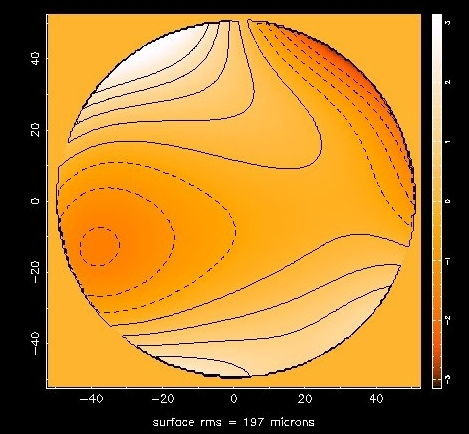
\includegraphics[width=.485\linewidth]{OOFgoodExample.jpg}}
\hfill
\subfloat[Unacceptable OOF solution.\label{fig:badOOFsolution}]
{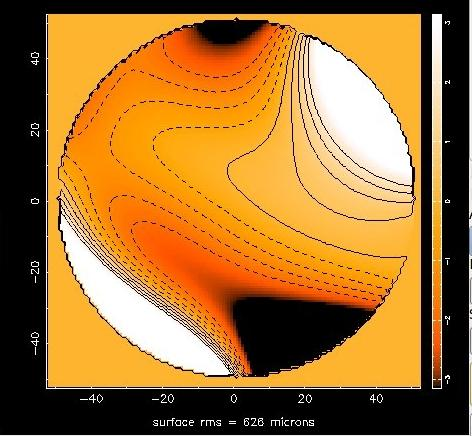
\includegraphics[width=.485\linewidth]{badoof.jpg}}
\caption[Comparison of AutoOOF solutions]
{Figure~\ref{fig:goodOOFsolution} shows broad features ($\pm 1.5$ radians
of phase) with a surface rms of 197 $\mu$m.  Figure~\ref{fig:badOOFsolution} shows
steep contour lines ($\pm 15$ radians of phase) and a surface rms of 626 $\mu$m.
This is likely the result of poor quality raw data and should not be used.} 
\label{fig:OOFsolution}
\end{center}
\end{figure}

%\vspace{-5mm}

\subsubsection{AutoOOF Raw Data}

Although an \gls{OOF} solution may appear to be reasonable (e.g.,
Figure~\ref{fig:goodOOFsolution}) it may also be invalid if it was derived
from a bad set of raw data.  Sending such a solution to the active surface could
degrade performance.  Therefore, observers should always check the quality of the
raw AutoOOF data in order to determine whether their derived solutions are valid.
For a set of raw data to be considered valid, it should show the following
characteristics:

\begin{itemize}[itemsep=0pt]
\item Clear detections of the source in the raw data timestream at all focus positions.
\item Symmetrical left/right positive/negative pattern in all three raw data images.
\item Smooth features in all three raw data images.  Sharp edges or stripes indicate
hardware/software glitches or excessive winds.
\end{itemize}

The AutoOOF raw data can be viewed by selecting the \dq{raw data} radio button in the
upper--right section of the OOF Subtab of the Data Display. Each column represents one focus
position.  The top row is the raw timestram data from the receiver, the second row
has the baselines removed, and the bottom row shows the corresponding beam maps.
See Figure~\ref{fig:rawOOFdata} for a comparison of acceptable and unacceptable
raw AutoOOF data.

\newpage

\begin{figure}[!h]
\begin{center}
\subfloat[A plot of the raw \gls{OOF} data on a fairly clean \gls{Kaband}/\gls{CCB} dataset.
\label{fig:goodOOFdata}]
{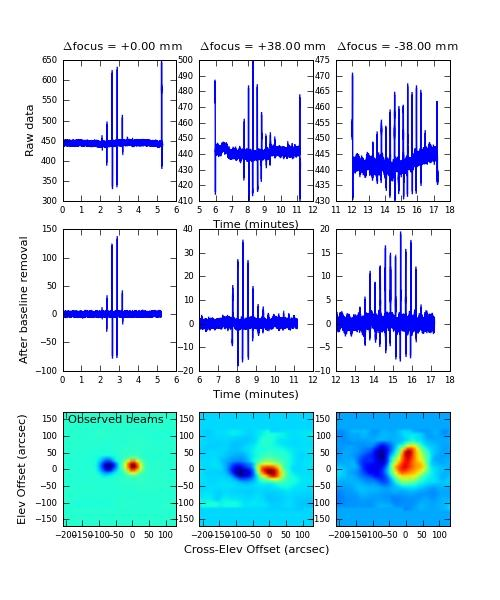
\includegraphics[width=.485\linewidth]{goodOOF.jpg}}
\hfill
\subfloat[A plot of raw \gls{OOF} data on a source which is too faint.
\label{fig:badOOFdata}]
{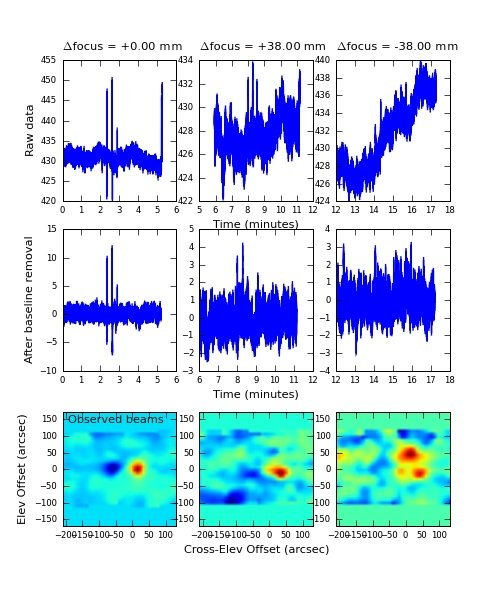
\includegraphics[width=.485\linewidth]{badOOF.jpg}}
\caption[Comparison of AutoOOF raw data]
{A comparison of acceptable and unacceptable AutoOOF raw data.}
\label{fig:rawOOFdata}
\end{center}
\end{figure}


\subsubsection{Selecting the Zernike order to fit}

By default, AutoOOF will halt processing after the fifth-order Zernike (z5) solution
has been computed. The z5 solution is suitable for most conditions and is generally what
observers should expect to use. A more agressive sixth-order (z6) fit may also be
derived at the cost of a few additional minutes of processing time.  This is usually
unnecessary and should only be done on bright calibrators under favorable weather
conditions. See \S~\ref{sec:OOFprocessing} for information on how to change the maximum
order of fit to process.

Occasionally, it may be necessary to occasionally drop to a lower order of fit if the
following features are seen:

\begin{itemize}[leftmargin=*]
\item {\bf Large excursions} over a significant area of the dish edge in the \gls{OOF}
solution.
\item {\bf Regularly spaced features} around the circumference of the dish at higher
order fits in the \gls{OOF} solution.
\item {\bf Anomalous values in the pointing/focus \gls{LPC}/\glspl{LFC}} for one
particular solution, or a significant jump in \glspl{LPC} above a certain Zernike fit
order.  For example, if the focus (LPCy) values for the z3--z4 solutions are around $-3mm$,
then abruptly jump to $+10mm$ for the z5 solution, then it would be prudent to assume that
some or all of the solutions may be invalid.  It may be possible to determine which solutions
are valid by examining the fitted beam maps for obvious artifacts or deviations from the
observed beams (see Figure~\ref{fig:fittedoofmap}).
\end{itemize}

\newpage

\begin{center}
\noindent\begin{minipage}[t]{0.48\linewidth}
\vspace{0pt}
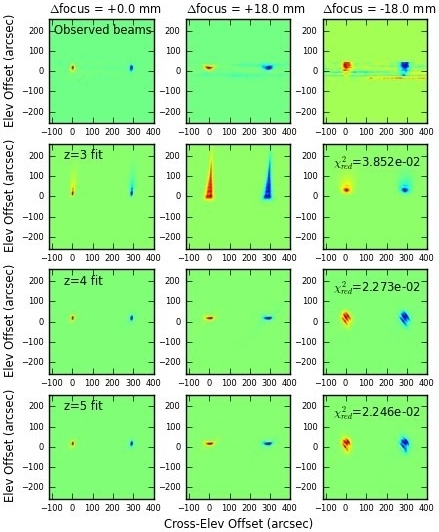
\includegraphics[width=\linewidth]{fittedoofmap_crop.jpg}
\end{minipage}
\hspace{0.025\linewidth}
\begin{minipage}[t]{0.36\linewidth}
\vspace{0pt}
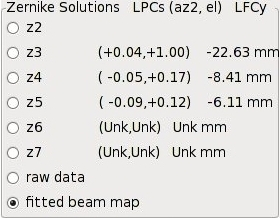
\includegraphics[width=\linewidth]{fittedoofmap_lpc.jpg}
\setlength{\abovecaptionskip}{0pt}\setlength{\belowcaptionskip}{0pt}
\captionof{figure}[AutoOOF fitted beam maps indicating a bad solution]
{The AutoOOF fitted beam maps (left). The observed beams are plotted on the top row
with the z3, z4 and z5 fits to the observed beams plotted below. The z3
solution (2$^{\text{nd}}$ row down) shows an obvious artifact and should not be used.
Also note the significant jump in \glspl{LPC} and the \gls{LFC} between the z3 and
z4 solutions (above).
\label{fig:fittedoofmap}}
\end{minipage}
\end{center}

\vspace{-2.5mm}
\subsubsection{Sending a Solution to the Active Surface}
\vspace{-2.5mm}

When you are ready to accept the solution being displayed it will need to be manually
sent to the active surface.  It is recommended that when sending the solutions, you use
the yellow button labeled
\astridyellowbutton{Send Selected Solution with Point and Focus Corrections}.
If you use this option, you do not have to perform a Peak or Focus after an AutoOOF.
It is still good practice to Peak and Focus at the beginning of your observing session
unless you are using the \gls{Wband} 68--92~GHz recevier (see Chapter~\ref{chap:wband}).
Subsequent pointing and focus corrections may be computed via AutoOOF.

Many high frequency observers will perform Peak scans immediately following
an AutoOOF to verify the surface solution (see \S~\ref{sec:oof_strategy}).
If the solution is satisfactory the \glspl{LPC} and \gls{LFC} from Peak/Focus
scans should agree with values from the \gls{OOF} solution, there should be no significant
sidelobes visible in the peak scans, and Peak scans should also yield the expected
beam \gls{FWHM}. If in doubt, you may disable \gls{OOF} corrections by pressing
\astridbutton{Zero and Turn Off Thernal Zernike Solution} in order to compare
Peak scans with and without \gls{OOF} corrections.

\subsubsection{OOF Processing Options}\label{sec:OOFprocessing}
\vspace{-2.5mm}

Deriving the sixth-order Zernike (z6) solution will require a few additional minutes of
processing time and for the user to manually change the maximum order of fit to process
in the following way:

\begin{center}
\noindent\begin{minipage}[t]{0.19\linewidth}
\setlength{\abovecaptionskip}{0pt}
\setlength{\belowcaptionskip}{0pt}
\vspace{0pt}
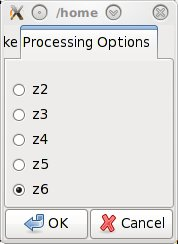
\includegraphics[width=0.73\linewidth]{OOFprocessing_options.jpg}
\captionof{figure}[OOF Processing Options]
{OOF Processing Options.
\label{fig:OOFprocessing}}
\end{minipage}
\begin{minipage}[t]{0.7\linewidth}
\vspace{0pt}
\begin{enumerate}[label=\bfseries{Step \arabic*.},leftmargin=*,itemsep=0pt]
\item Select the OOF Subtab of the Data Display.
\item Select {\btt Tools}$\rightarrow${\btt Options...} from the drop--down menu.
\item Select the maximum order of fit to process from the \newline
\dq{Processing Options} tab of the pop--up window (Figure~\ref{fig:OOFprocessing}).
\item[{\bf NOTE:}] All changes must be made {\bf before submitting the \gls{SB}}
containing the \textbf{\textcolor{pythonKeywords}{AutoOOF}()} function in order to take
effect.  You may also repeat processing after making any changes by pressing
\astridbutton{Reanalyze OOF (Online Only)}.
\end{enumerate}
\end{minipage}
\end{center}

%%%%%%%%%%%%%%%%%%%%%%%%%%%%%%%%%%%%%%%%%%%%%%%%%%%%%%%%%%%%%%%%%%%%%%%%%%%%%%%%%%%%%

\newpage

\subsection{Continuum Data Display}

Continuum data taken with the \gls{GBT} that are not part of pointing and focus
scans will show up in plots under the Continuum Tab
(see Figure~\ref{fig:astridcontinuum}).  This will show the uncalibrated continuum
data as a function of time only.

\begin{figure}[!h]
\begin{center}
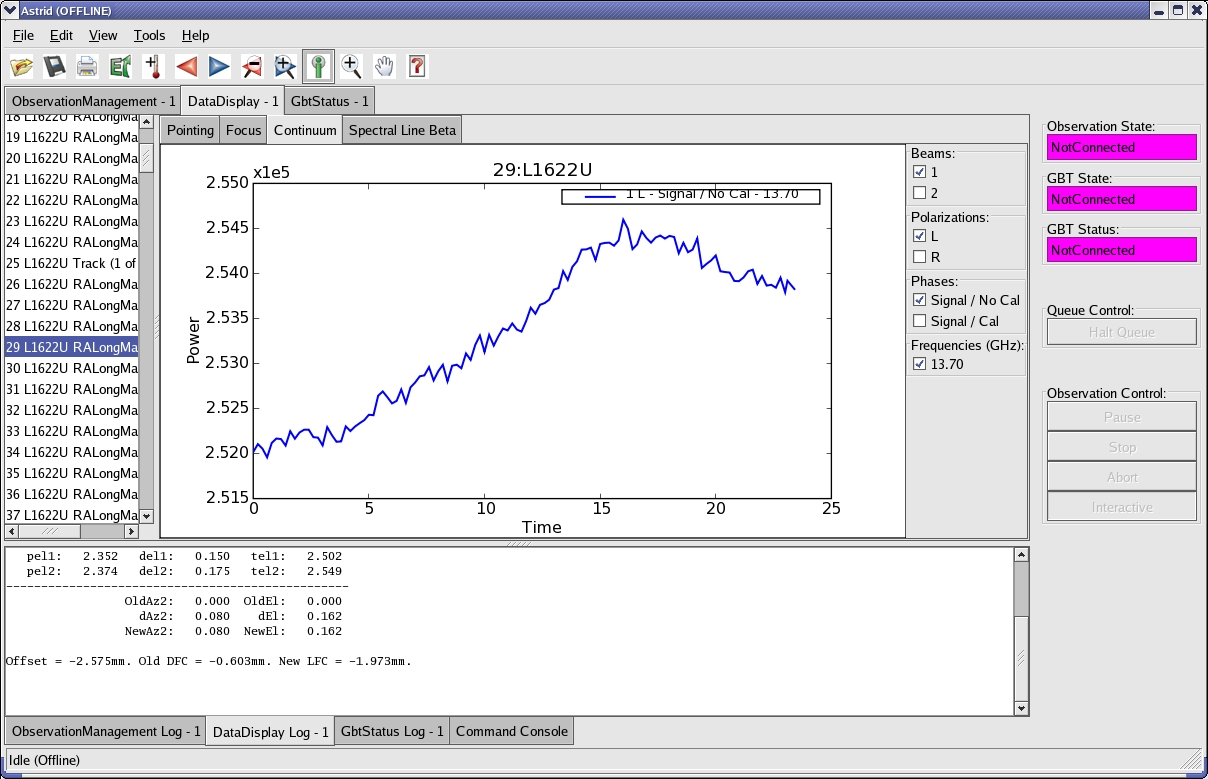
\includegraphics[width=0.9\linewidth]{AstridDataDisplayTabContinuum.jpg}
\caption[The Continuum subtab of the Astrid Data Display]
{The Continuum subtab of the \gls{Astrid} Data Display.\label{fig:astridcontinuum} }
\end{center}
\end{figure}

\vspace{-5mm}

\subsection{Spectral Data Display}\label{sec:spectral_data_display}

The Spectral Line Display was a tool originally designed for browsing the previous
\gls{GBT} Spectrometer spectral line data.  Although this tool can provide limited
\gls{VEGAS} information, there is a separate, more flexible web-based display intended
for \gls{VEGAS}. See \S~\ref{sec:vegasdisplay} for more details.

When viewing data online, the most recent integration is plotted automatically.
Individual integrations may be selected and viewed offline. See
Figure~\ref{fig:astridspectralline} for an example of the spectral line data display.
The spectra displayed are raw data and no calibration has been applied to them.
As spectra are plotted, information about each plot is printed in the console window.
Each line is color coded to match the color of that spectrum in the plotting window. In
addition, some of the information for the very first spectra are used to annotate the
plot. The plot title is parsed as project\_name:scan\_number:integration\_number.
For offline usage, the desired integration can be selected either using the up/down arrows,
or by typing in a value in the edit box.

All user interaction for this plugin occurs in the right-hand side options panel. The
check boxes allow selection of spectra to plot via astronomical variables: Beams,
Polarizations, \gls{IF} Numbers, and Phases.
The options panel also includes three buttons and a radio box for plot viewing. The
\dq{Views} radio box offers options for plotting the bandpass vs. Channels or Sky
Frequency. The \astridbutton{Keep Zoom} toggle button will maintain the current zoom, even
as new spectra are plotted. Using the unzoom command (mouse right-click, or via the
tool bar) will return the plot to its original scale. The \astridbutton{Overlay} toggle
button can be used to overplot spectra from different integrations or scans.
Finally, the \astridbutton{Clear} button erases the plot.

\newpage

\begin{figure}[!h]
\begin{center}
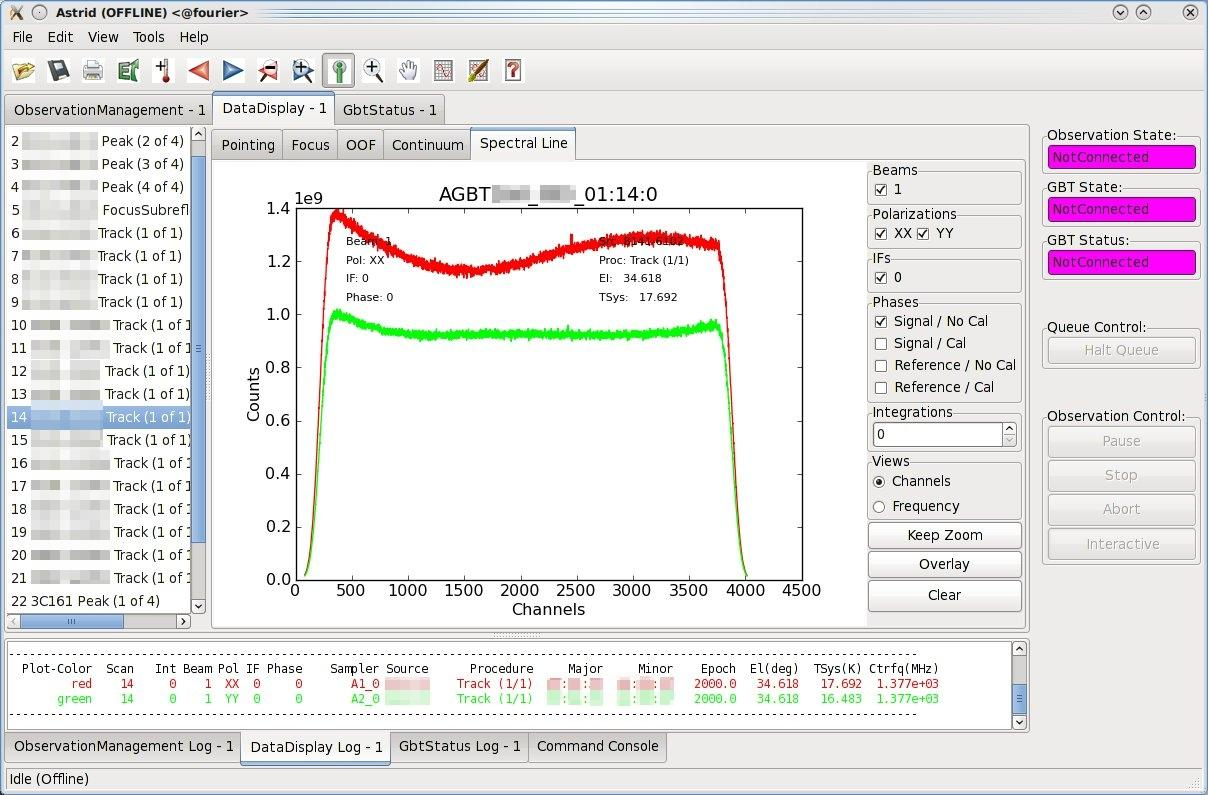
\includegraphics[width=0.9\linewidth]{AstridSpectralDisplay.jpg}
\caption[The Spectral Line subtab of the Astrid Data Display]
{The Spectral Line subtab of the \gls{Astrid} Data Display. 
\label{fig:astridspectralline} }
\end{center}
\end{figure}


\subsection{The Data Display Plotting Panel Toolbar}

The plotting panel toolbar allows user interactions with plots in the display window and
is located near the top of the Astrid Screen.  The following features are available:

\begin{itemize}
\item[
\includegraphics{DTopen.jpg}] {\bf Open:} Allows the user to open a previously
saved session.  This has the same functionality as file $\rightarrow$ open described
in \S~\ref{sec:workingOffline}.
\item[
\includegraphics{DTsave.jpg}] {\bf Save:} Allows the user to save output from the
data display log as a text file.
\item[
\includegraphics{DTprint.jpg}] {\bf Print (DO NOT USE):} Please use the \dq{export}
function instead.
\item[
\includegraphics{DTexport.jpg}] {\bf Export:}  Allows the user to save the figure
displayed in the plotting panel to a file.  The name must have an extension of either
.png, .ps or .eps.
\item[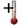
\includegraphics{DTunfreeze.jpg}] {\bf Unfreeze:} Not applicable to Astrid general
use. Unfreezes the processing of commands via the command line and intended for use in
conjunction with the \dq{freeze} command.
\item[
\includegraphics{DTundo.jpg}] {\bf Undo:} Undoes your last command.
\item[
\includegraphics{DTredo.jpg}] {\bf Redo:} Redoes your last command.
\item[
\includegraphics{DTunzoom.jpg}] {\bf Unzoom:} Undoes a previously executed zoom.
\item[
\includegraphics{DTrezoom.jpg}] {\bf Rezoom:} Redoes a previously executed zoom.
\item[
\includegraphics{DTinfo.jpg}] {\bf Info Tool:} Selecting the info tool allows the
user to use the mouse pointer to focus in/out among the available subplots (e.g., peak
scans). Left-clicking the mouse brings a subplot into focus (hiding the other subplots).
Right-clicking the mouse on the focused plot will show all subplots. If there is only
one subplot, the info tool simply displays the mouse xy coordinates.
\item[
\includegraphics{DTzoom.jpg}] {\bf Zoom Tool:} Selecting the zoom tool allows the
user to use the mouse pointer for zooming in on a particular area of the plot.
Left-clicking the mouse will zoom in. Right-clicking the mouse will zoom out.
\item[
\includegraphics{DTpan.jpg}] {\bf Pan Tool:} Allows the user to use the mouse
pointer to pan around the selected subplot.  Left-clicking the mouse and holding the left
button down will pan around the subplot. Right-clicking restores the original view.
\item[
\includegraphics{DTgrid.jpg}] {\bf Grid Tool:} Turns on the plot grid.
\item[
\includegraphics{DTplotedit.jpg}] {\bf Plot Edit Tool:} Allows the user to edit
plot labels, colors, and title. Clicking on "Advanced Options" brings up an additional
dialog which contains options for transparency, legend placement, and ordering of plots.
Colors may be entered as hex codes or selected by clicking on the colored button to the
right of the text field. Plots can only be reordered within their subplot - i.e., Y1
lines will always be below Y2 lines. Legend location can be specified with simple
strings (e.g., "upper right") or coordinates 0-1 along the plot edges. If a string is
chosen it will be used in place of any coordinates.
\item[
\includegraphics{DTusermanual.jpg}] {\bf User Manual:} Displays the DEAP user
manual.

\end{itemize}


\subsection{Use of Plotting Capabilities}

A User Manual is available at
\htmladdnormallink{http://deap.sourceforge.net/help/index.html}
{http://deap.sourceforge.net/help/index.html}
that describes all the plotting functionality available in \gls{GFM}. There is also a
plotting Tutorial that illustrates the plotting capabilities by example which is
available at
\htmladdnormallink{http://deap.sourceforge.net/tutorial/index.html}
{http://deap.sourceforge.net/tutorial/index.html}.


%++++++++++++++++++++++++++++++++++++++++++++++++++++++++++++++++++++++++++++
\newpage

\section{The CLEO Utilities}\label{sec:cleo}

The \glsfirst{CLEO} system provides a large number of utilities for monitoring
and controlling the GBT hardware systems. Some of these are quite useful for observers,
although most are intended for expert users and \gls{GBT} staff.

Useful help messages pop up when you hover the mouse over any \gls{CLEO} widget for a
few seconds.  Documentation is also available on the following web pages, but is somewhat
out of date, so its best to consult your \gls{GBT} \dq{friend} for details.
\begin{itemize}
\item \htmladdnormallink
{http://www.gb.nrao.edu/$\sim$rmaddale/GBT/CLEOManual/index.html}
{http://www.gb.nrao.edu/~rmaddale/GBT/CLEOManual/index.html}
\item \htmladdnormallink
{http://www.gb.nrao.edu/$\sim$rmaddale/GBT/CLEOManual/tableofcontents.html}
{http://www.gb.nrao.edu/~rmaddale/GBT/CLEOManual/tableofcontents.html}.
\end{itemize}

\noindent The following section describes just a few \gls{CLEO} utilities that are
useful for observers.

\subsection{Starting CLEO}

\noindent\begin{minipage}[b]{0.29\linewidth}
\vspace{0pt}
\captionsetup{
  justification=raggedright,
  singlelinecheck=false
}
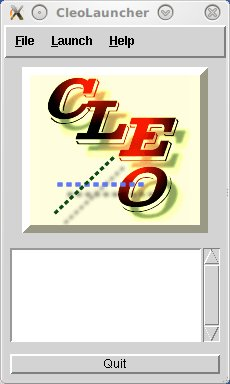
\includegraphics[width=\linewidth]{cleoLauncher.jpg}
\captionof{figure}[The Cleo Launcher]
{The Cleo Launcher.
\label{fig:cleoLauncher}}
\end{minipage}
\hfill
\noindent \begin{minipage}[b]{0.685\linewidth}
\vspace{0pt}
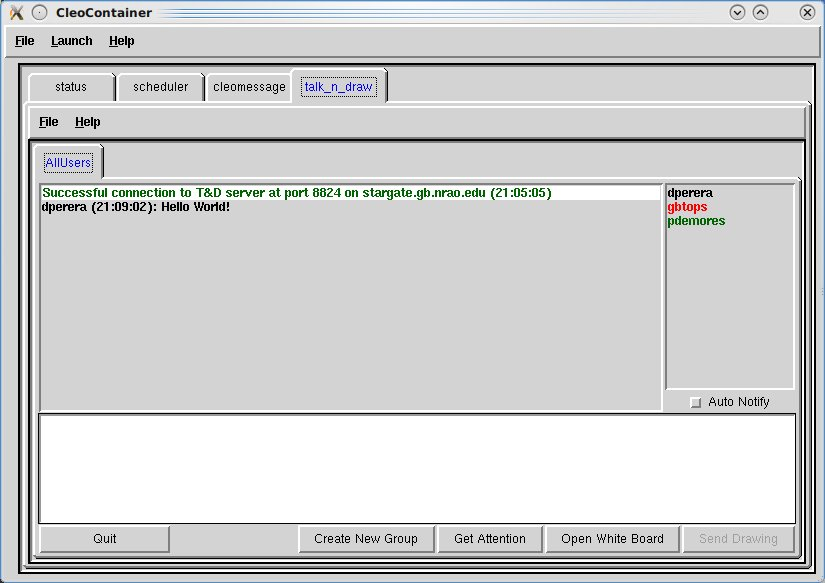
\includegraphics[width=\linewidth]{CLEOtalkAndDraw.jpg}
\captionof{figure}[CLEO Talk and Draw]
{The \gls{CLEO} Talk and Draw application launched as a tab of the Cleo Container.
\label{fig:CLEOtalkanddraw}}
\end{minipage}

To start \gls{CLEO}, log in to any Linux workstation in Green Bank, open a terminal 
window, and type {\tt cleo}.  A \dq{Cleo Launcher} window will appear
(see Figure~\ref{fig:cleoLauncher}).  Click on the {\btt \underline{L}aunch} menu
to get a list of programs that can be run.  Remote observers working via \gls{VNC} may
prefer to use \dq{Cleo Container} which launches and displays \gls{CLEO} applications
as tabs within a single window.  Cleo Container can be opened from the terminal by typing 
{\tt cleo cleocontainer} or from the Cleo Launcher via\\
{\btt \underline{L}aunch} $\rightarrow$ {\btt \underline{C}leo Container...}

\newpage

\subsection{Talk and Draw}\label{sec:talkanddraw}
{\btt \underline{L}aunch} $\rightarrow$ {\btt \underline{O}bserver
Tools} $\rightarrow$ {\btt Talk and Dra\underline{w}}

Launching \dq{Talk and Draw} will open a window that allows communication
with all other users of the same application including the \gls{GBT} operator
(see Figure~\ref{fig:CLEOtalkanddraw}). Messages typed in the white text box
near the bottom of the screen will become visible to other users after pressing
the \dq{Enter} key.

Users may also create private groups via the \cleobutton{Create New Group} button and
inviting other users to join.  The private session will be accessible through a new
tab next to the default \dq{AllUsers} tab.  Users may then send messages within
their newly created group or to \dq{AllUsers} (including the operator) by selecting
the relevant tab and entering a message.



\subsection{Scheduler and Skyview}\label{sec:cleo_scheduler}
{\btt \underline{L}aunch} $\rightarrow$ {\btt \underline{O}bserver
Tools} $\rightarrow$ {\btt Sc\underline{h}eduler \& Skyview...}

This displays a plot of the sky in Az/El coordinates as viewed from Green Bank as
shown in Figure~\ref{fig:CLEOskyview}.   One can import a catalog of source positions
to be displayed, or display one of the lists of standard calibration sources.
By default it displays solar system objects. For example, to display sources listed in
the standard \gls{Astrid} \dq{xband\_pointing} catalog press

\begin{itemize}[leftmargin=*]
\item \cleobutton{Catalog...}$\rightarrow$\cleobutton{Add/Select/DeSelect Catalogs...}%
$\rightarrow$\cleobutton{xband\_pointing}$\rightarrow$\cleobutton{Apply}$\rightarrow$\cleobutton{OK}
\end{itemize}

If one selects \cleobutton{Schedule} (button at upper right), one may enter a date and time
and display the sky for that time.  It shows the corresponding \gls{LST}, and moving
the cursor on the plot displays the RA/Dec and Az/EL under the cursor. This is very
useful for planning observations. There is also a \cleobutton{Real Time} option in which the
location of objects and the direction the \gls{GBT} is pointed are displayed for the
current time.

\begin{figure}[!h]
\setlength{\abovecaptionskip}{0pt}\setlength{\belowcaptionskip}{0pt}
\begin{center}
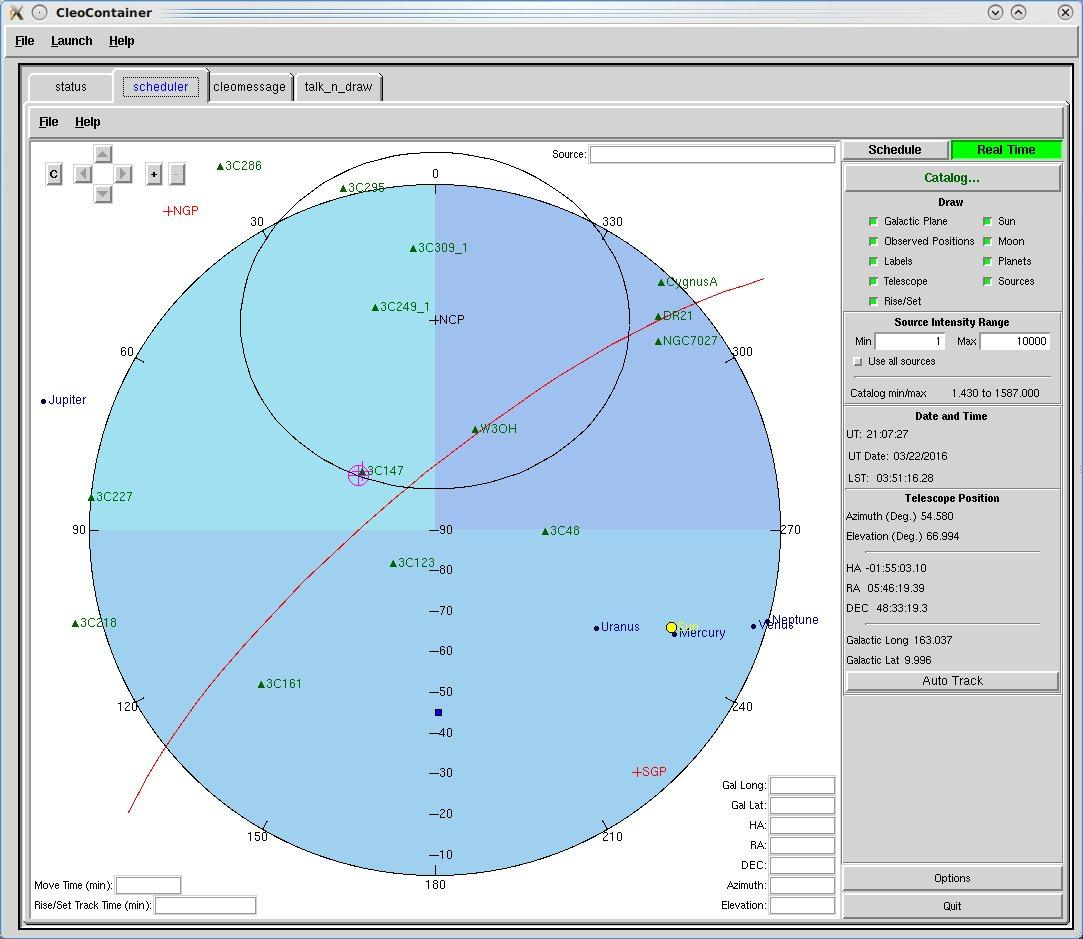
\includegraphics[width=0.6\linewidth]{CLEOscheduler.jpg}
\caption[CLEO Scheduler \& Skyview]
{The \gls{CLEO} Scheduler \& Skyview application.
\label{fig:CLEOskyview}}
\end{center}
\end{figure}
\newpage

\subsection{Status}
{\btt \underline{L}aunch} $\rightarrow$ {\btt S\underline{t}atus...}

This displays the status of many \gls{GBT} systems all on one screen as shown in
Figure~\ref{fig:CLEOstatus}. While very useful, it is not recommended for use remotely because it 
is a heavy user of computing resources.  For remote observing, it is
recommended to use the Astrid GbtStatus display (See Section~\ref{sec:astridstatus}).

\begin{figure}[!h]
\begin{center}
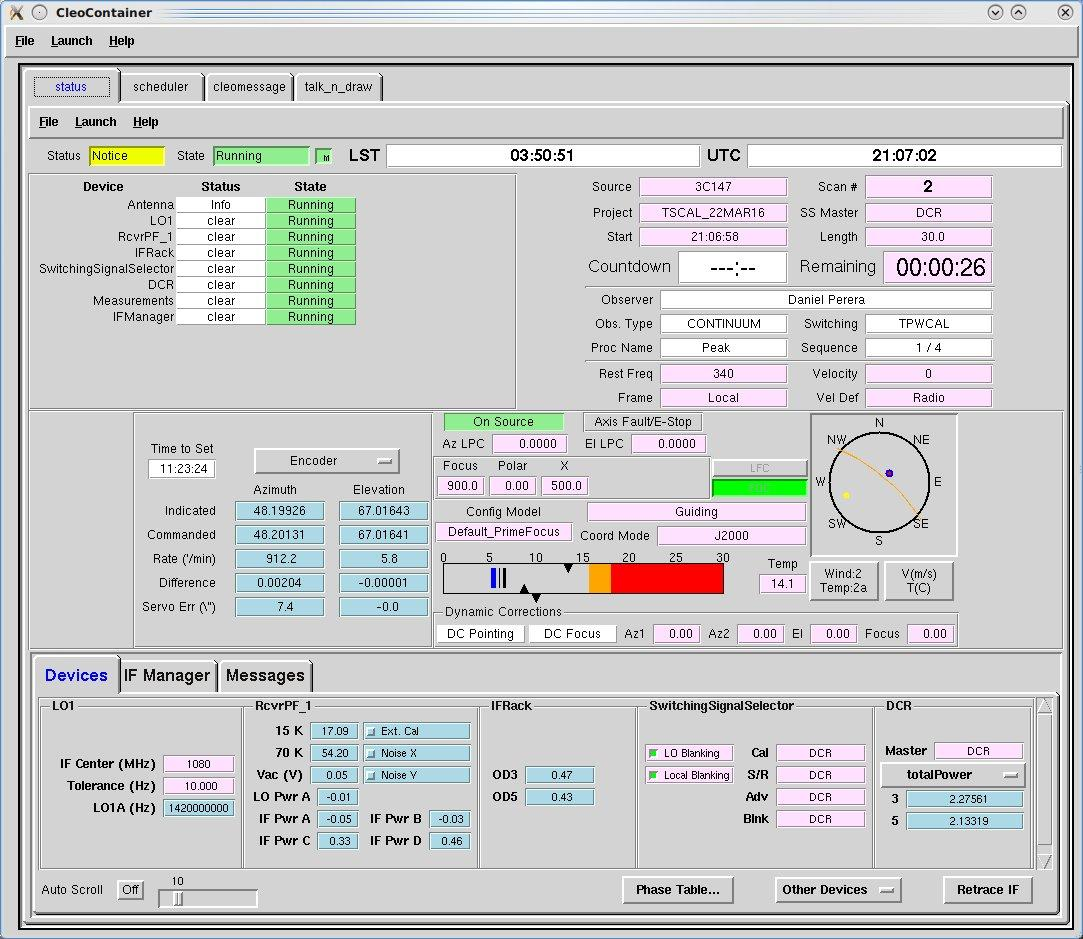
\includegraphics[width=0.7\linewidth]{CLEOstatus.jpg}
\caption[CLEO Status]
{The \gls{CLEO} Status application.
\label{fig:CLEOstatus}}
\end{center}
\end{figure}

\vspace{-1cm}

\subsection{Messages}
{\btt \underline{L}aunch} $\rightarrow$ {\btt \underline{M}essages...}

This shows all system status messages as shown in Figure~\ref{fig:CLEOmessages}.
It's often useful to identify problems that might arise with any of the \gls{GBT} devices.

\begin{figure}[!h]
\begin{center}
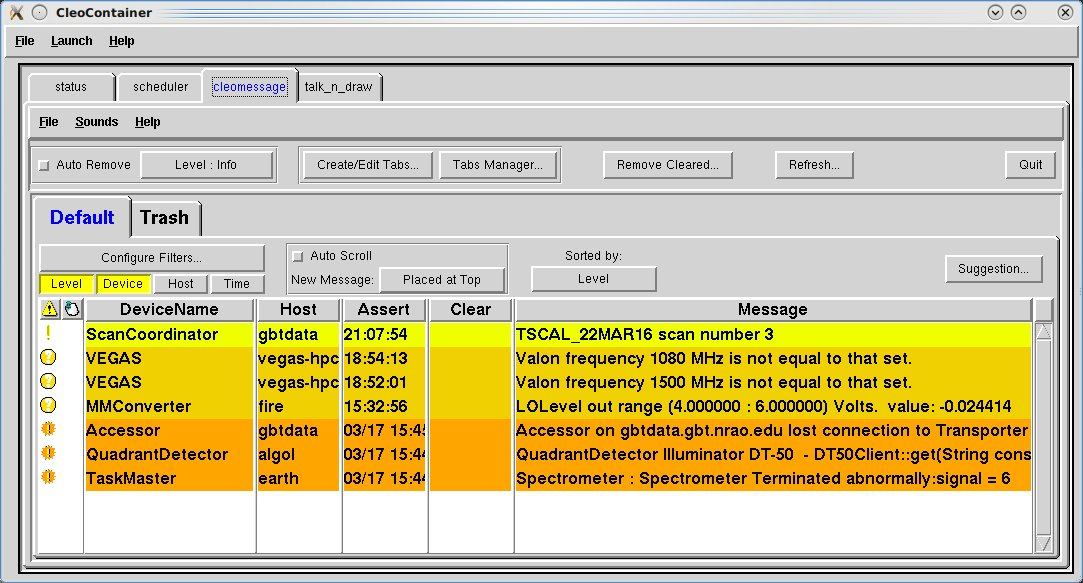
\includegraphics[width=0.5\linewidth]{CLEOmessages.jpg}
\caption[CLEO Messages]
{The \gls{CLEO} Messages application.
\label{fig:CLEOmessages}}
\end{center}
\end{figure}


%===========================================================================

\newpage

\section {VEGAS Monitoring Tools}\label{sec:vegas_monitoring_tools}

\subsection {The VEGAS Data Display}\label{sec:vegasdisplay}
Observers are urged to use the real-time data display any time they are observing with
\gls{VEGAS} to monitor data quality in real time. The \gls{VEGAS} real-time data display
may be accessed by pointing a web browser to \htmladdnormallink
{http://vegasdisplay.gb.nrao.edu}
{http://vegasdisplay.gb.nrao.edu}
\begin{center}
(This URL is only accessible to machines inside the Green Bank observing network)
\end{center}

\vspace{-2.5mm}

\begin{figure}[!h]
\setlength{\abovecaptionskip}{0pt}\setlength{\belowcaptionskip}{0pt}
\begin{center}
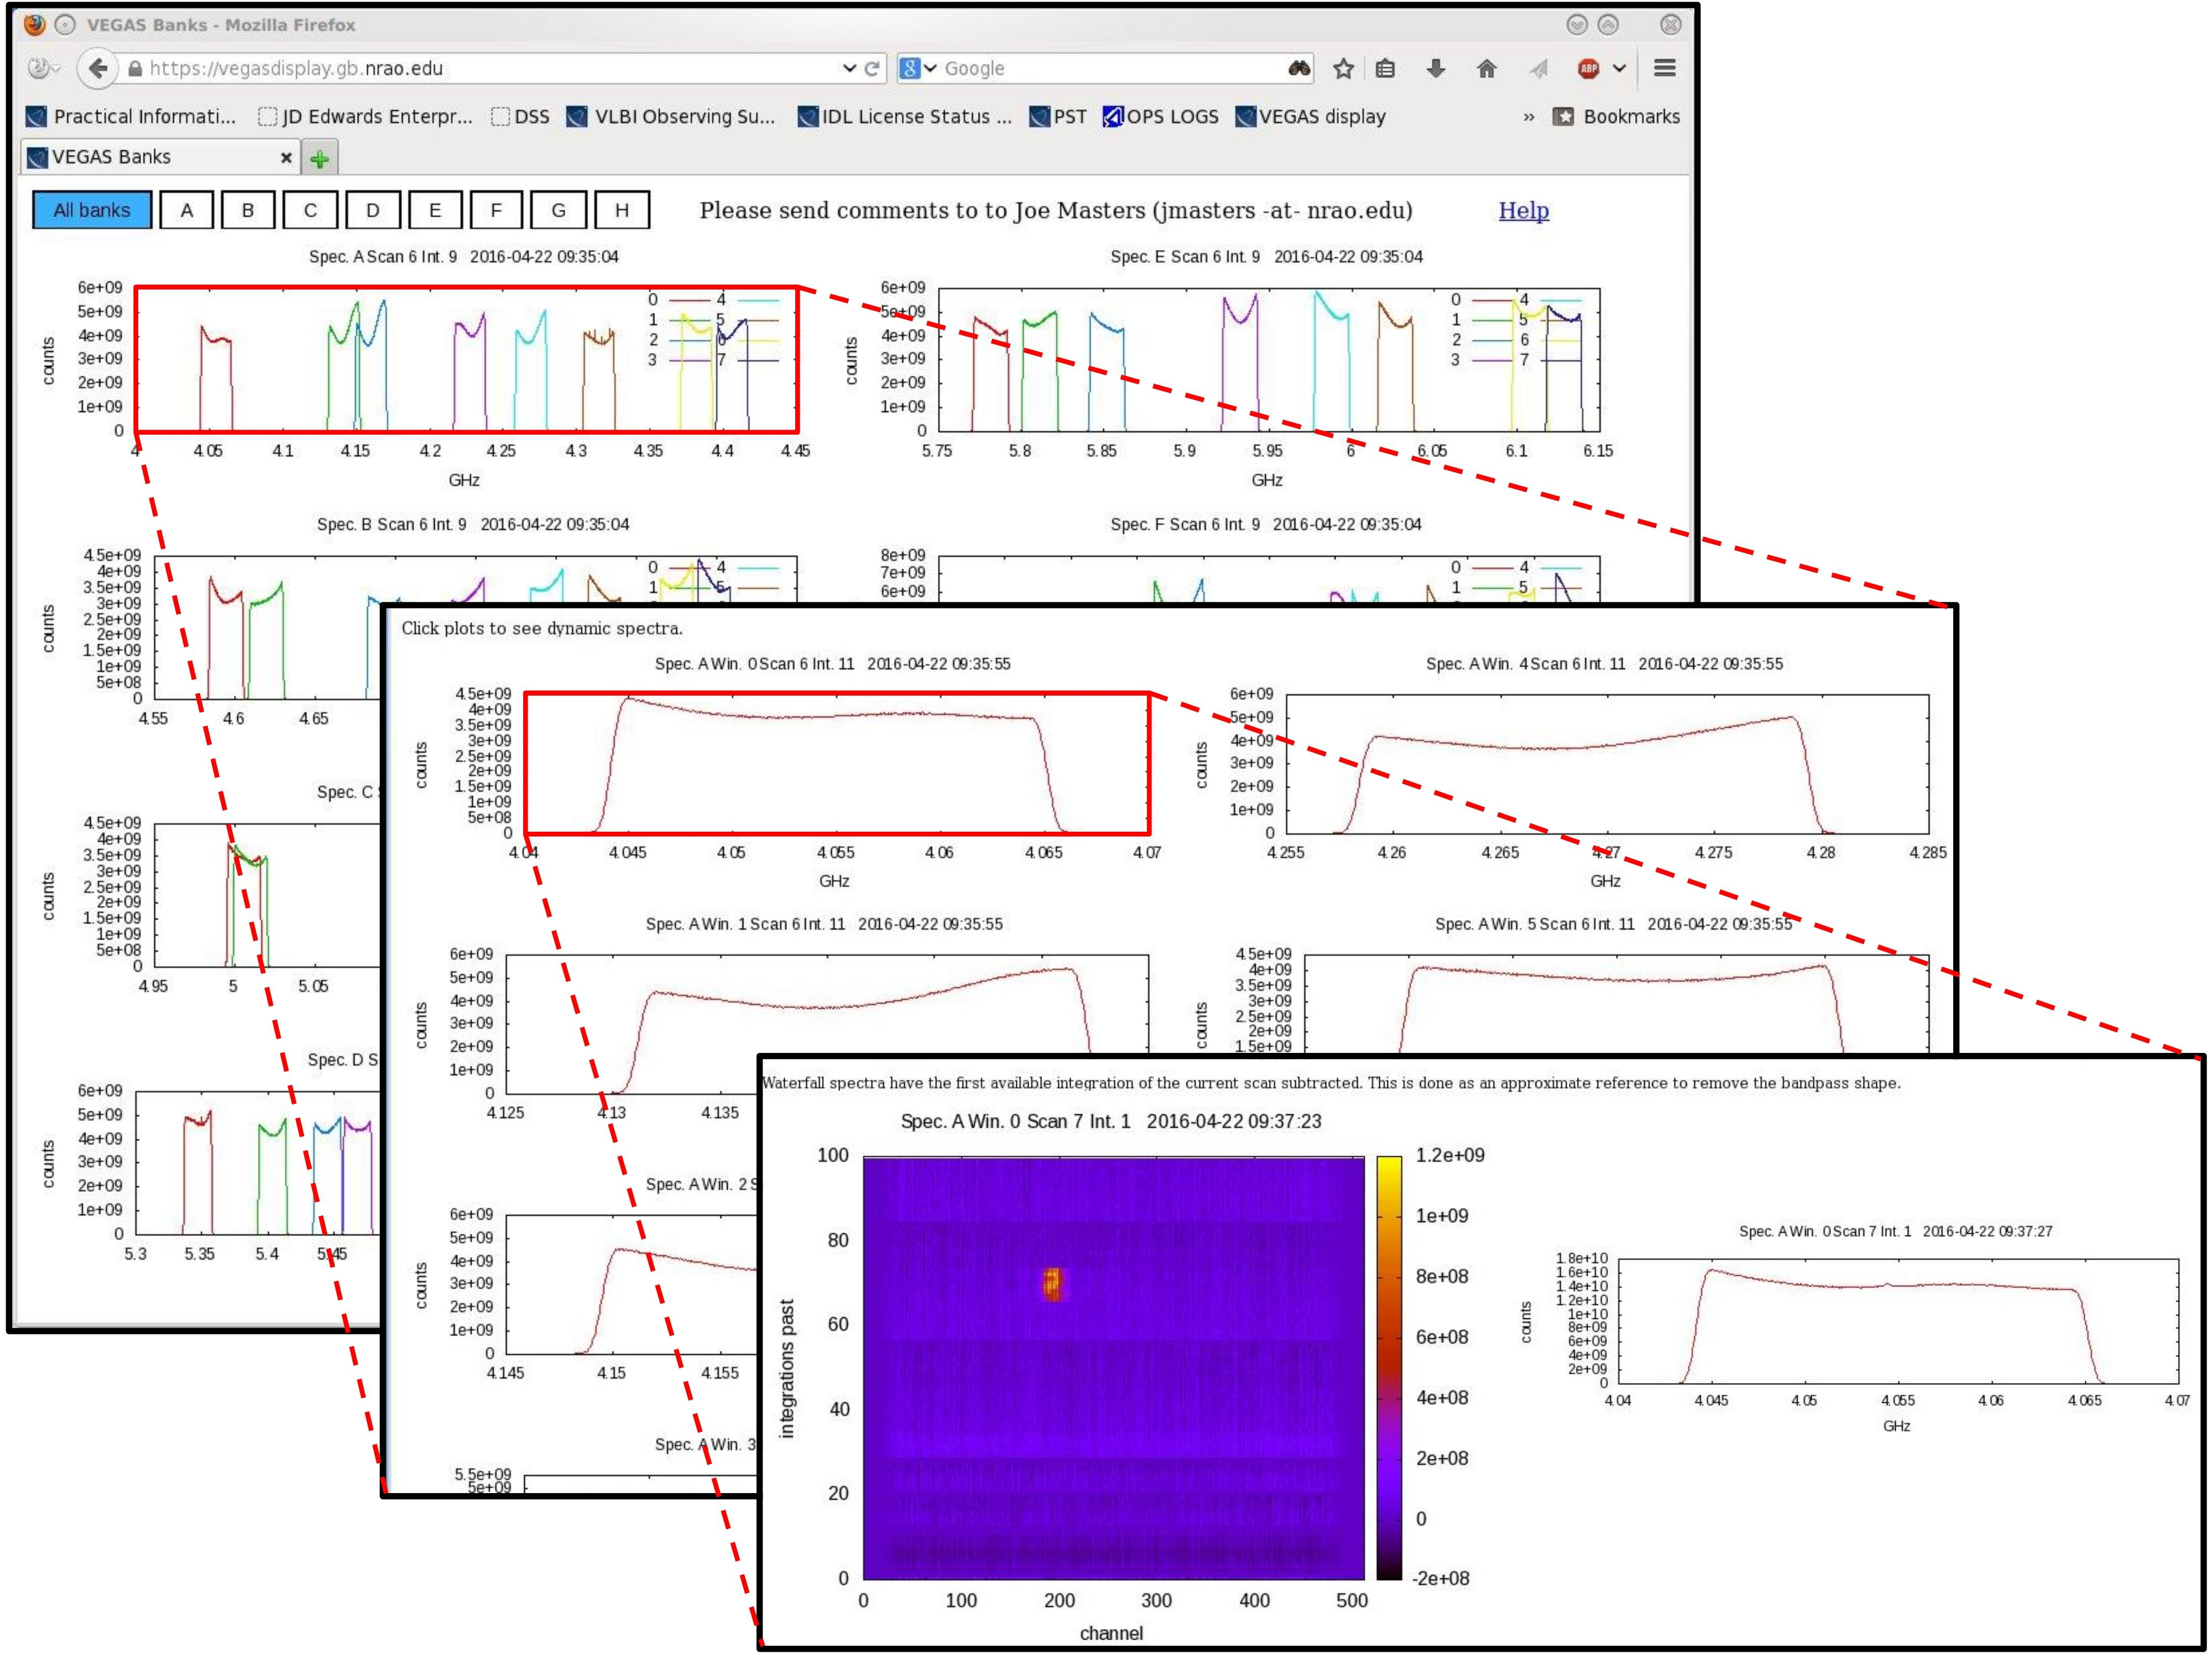
\includegraphics[width=\linewidth]{vegas_display_layers.jpg}
\caption[The VEGAS real-time data display]{The VEGAS real-time data display.
The first level displays data for each \gls{VEGAS} bank, the second level displays data for
each subband of a selected bank, and the third level displays a false color \dq{waterfall}
plot for a single selected subband.
\label{fig:vegas_real_time_display}}
\end{center}
\end{figure}

\vspace{-2.5mm}

\noindent This will bring up a display as shown in the top-left box of
Figure~\ref{fig:vegas_real_time_display} where each plot represents a bank of \gls{VEGAS}.
Subbands (if available) are color coded within each bank.
\begin{itemize}
\item Clicking on the plot for a \gls{VEGAS} bank or the boxes labelled
\dq{A}$\rightarrow$\dq{H} near the top of the screen will dislay total power in counts
vs. frequency for each subband of the selected bank. A maximum of eight subbands will
be displayed in the plots labelled \dq{Window 0$\rightarrow$7}.  If using a single band
mode of \gls{VEGAS}, then only \dq{Window 0} will display a bandpass.
\begin{itemize}
\item Clicking on a subband plot will display a false color \dq{waterfall} plot, building
up integration by integration.  The right hand plot of this new screen will also display
the bandpass of the latest integration.  Note that the waterfall plot will always rebin
data to 512 channels.
\end{itemize}
\end{itemize}


\newpage

\subsection{The VEGAS CLEO screen}\label{sec:vegas_cleo}


This can be launched via {\btt \underline{L}aunch} $\rightarrow$
{\btt \underline{B}ackends} $\rightarrow$ {\btt \underline{V}EGAS...} from the
\gls{CLEO} launcher (see \S~\ref{sec:cleo}). An example of the \gls{VEGAS}
\gls{CLEO} screen is shown in Figure~\ref{fig:vegas_cleo}.

\begin{figure}[!h]
\begin{center}
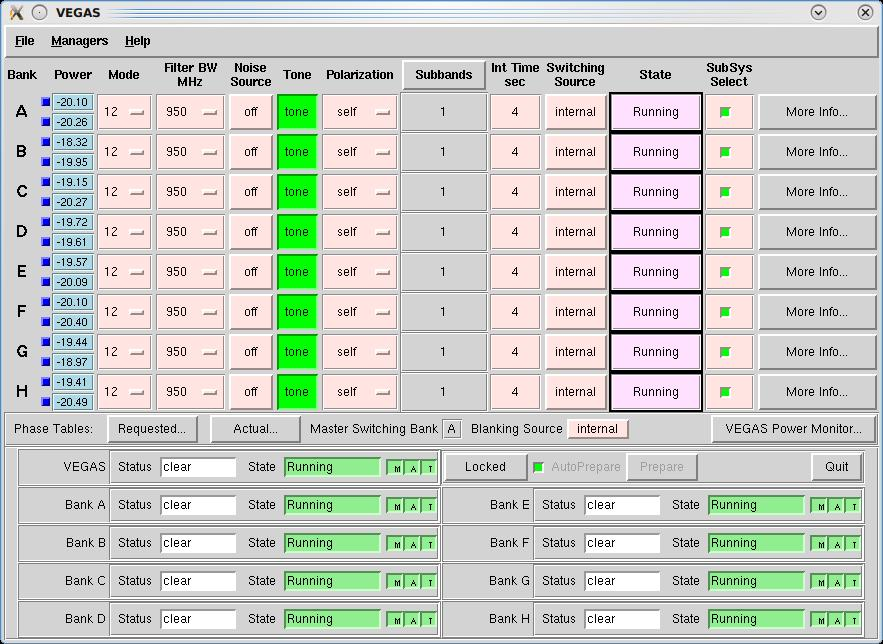
\includegraphics[width=\linewidth]{vegascleoscreen.jpg}
\caption[]{The VEGAS CLEO Screen \label{fig:vegas_cleo}}
\end{center}
\end{figure}

The \gls{VEGAS} \gls{CLEO} screen follows standard \gls{CLEO} conventions, and is fairly
self-explanatory. As for all backend screens, \gls{IFsys} information for a selected
bank can be displayed by clicking on the blue square to the right of the Bank label.

The \gls{VEGAS} \gls{CLEO} screen can be used to launch the \gls{VEGAS} Data Monitor (described
in the next section) by clicking on the \cleobutton{VEGAS Power Monitor...} button.

\newpage

\subsection{VEGAS Data Monitor}\label{sec:vegasdm}
The \gls{VEGAS} Data Monitor (VEGASDM) provides a real-time display of the current
total power level as measured by the \gls{VEGAS} \glspl{ADC}, as well as a histogram of
the distribution of \gls{ADC} counts.  VEGASDM may be launched by:

\begin{verbatim}
% source /home/gbt/gbt.bash (or .csh)
% VEGASDM
\end{verbatim}

or by clicking the \cleobutton{VEGAS Power Monitor...} button from the \gls{VEGAS} \gls{CLEO} screen.
The VEGASDM display will appear as in Figure~\ref{fig:vegasdm}

\begin{figure}[!h]
\begin{center}
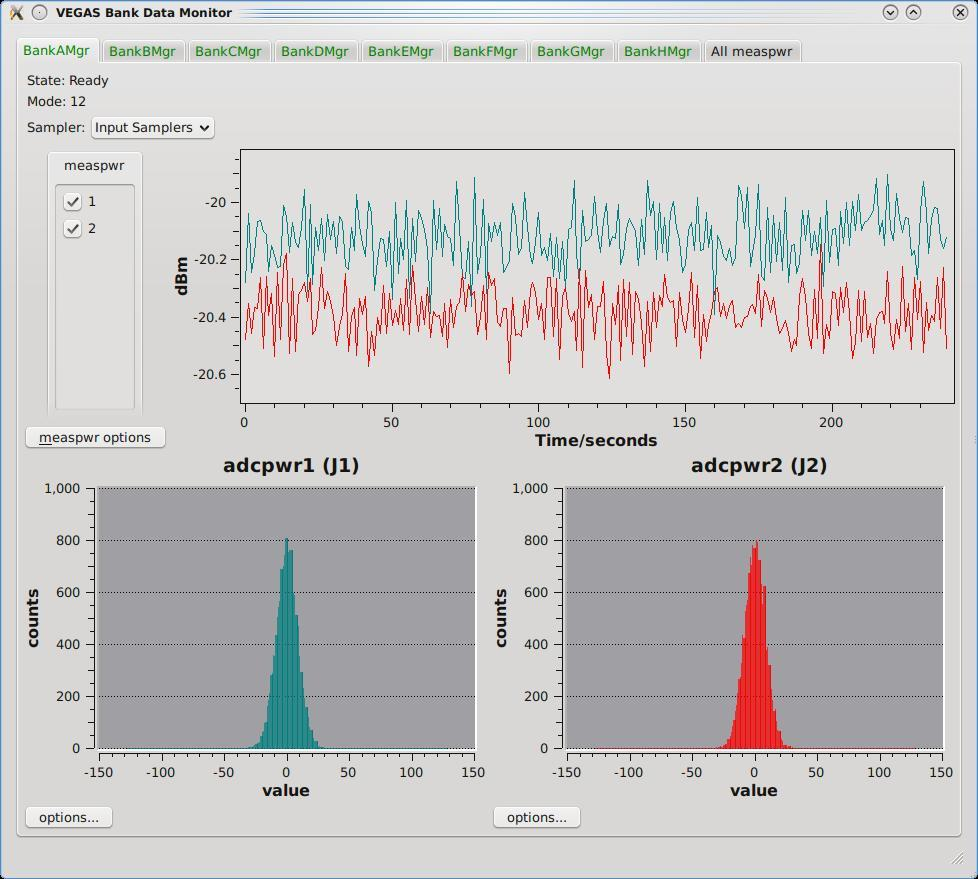
\includegraphics[width=0.85\linewidth]{vegasdatamonitor.jpg}
\caption[]{The VEGAS Data Monitor screen}
\label{fig:vegasdm} 
\end{center}
\end{figure}

VEGASDM has nine tabs, one for each Bank, and one overview tab. If a Bank is
active, the tab label will be green, otherwise it will be red. Each Bank tab
shows whether the Bank is in the running state, and what mode it is in. The
upper plot shows the total power from each polarization as a function of
time, while the lower two plots show the distribution of \gls{ADC} counts for
each polarization. If \gls{VEGAS} is balanced correctly, the \gls{ADC} counts should
be approximately Gaussian, centered around zero, with a full-width half
maximum of approximately 25--50 counts. If the \gls{ADC} counts are very centrally
peaked, there is not enough power going into \gls{VEGAS}, while if the \gls{ADC} counts
have peaks at +/- 127 counts, \gls{VEGAS} is being over-driven.

The final tab of VEGASDM gives an overview plot of the total power for all
eight banks on a single screen.




%\begin{figure}[!h]
%\begin{center}
%\subfloat[z6 fit with a large excursion near the bottom of the dish
%\label{fig:OOFZ6toZ5bad}]
%{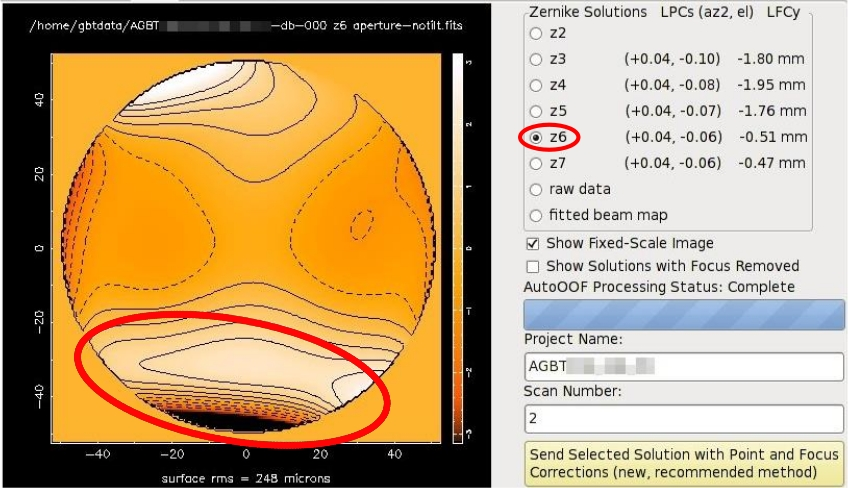
\includegraphics[width=.475\linewidth]{OOFZ6toZ5bad.jpg}}
%\hfill
%\subfloat[z5 fit no longer showing the large excursion
%\label{fig:OOFZ6toZ5good}]
%{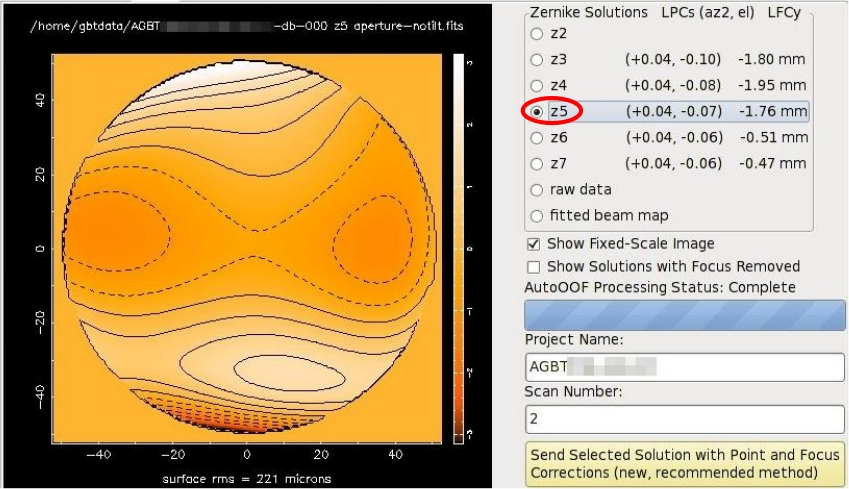
\includegraphics[width=.475\linewidth]{OOFZ6toZ5good.jpg}}
%\caption[Selecting the z5 AutoOOF solution]
%{An example of using a lower order z5 fit (figure~\ref{fig:OOFZ6toZ5good}) to
%correct for a large excursion ($\pm 5$ radians of phase) seen near the bottom of the dish in the
%z6 fit (figure~\ref{fig:OOFZ6toZ5bad}).  Also note the slight jump in derived focus LPCs
%from approximately -1.8 mm (z2--z5) to -0.5 mm (z6--z7).}
%\label{fig:OOFZ6toZ5correction}
%\end{center}
%\end{figure}

%\begin{figure}[!h]
%\begin{center}
%\subfloat[z7 fit showing repeating features.\label{fig:OOFZ7toZ6bad}]
%{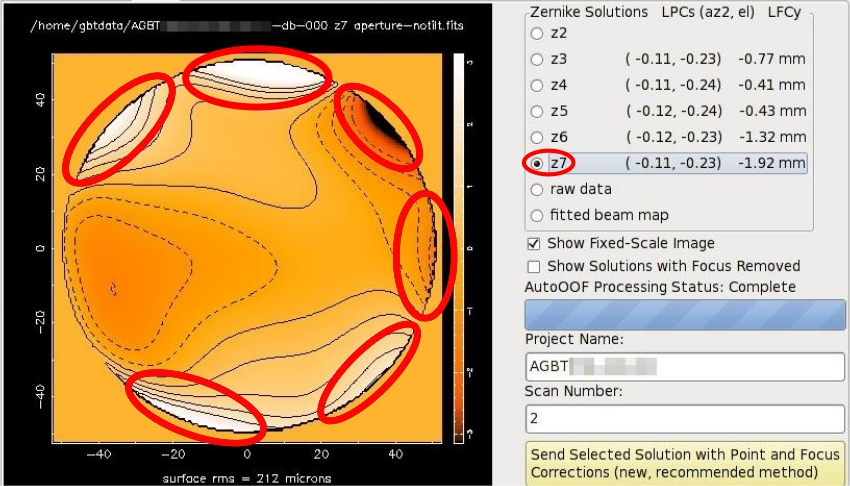
\includegraphics[width=.475\linewidth]{OOFZ7toZ6bad.jpg}}
%\hfill
%\subfloat[z6 fit no longer showing repeating features.\label{fig:OOFZ7toZ6good}]
%{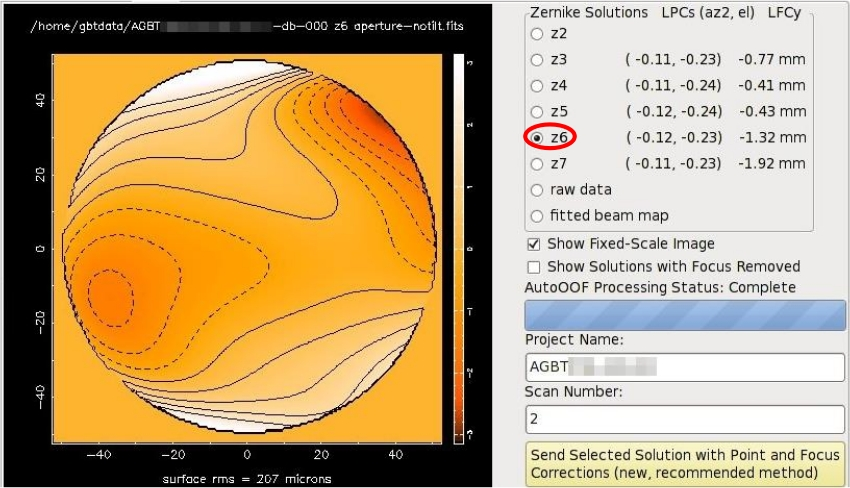
\includegraphics[width=.475\linewidth]{OOFZ7toZ6good.jpg}}
%\caption[Selecting the z6 AutoOOF solution]
%{An example of using a lower order z6 fit (figure~\ref{fig:OOFZ7toZ6good}) to
%correct for the repeating features seen in the z7 fit (figure~\ref{fig:OOFZ7toZ6bad}).}
%\label{fig:OOFZ7toZ6correction}
%\end{center}
%\end{figure}
